
%
%  $Description: Author guidelines and sample document in LaTeX 2.09$ 
%
%  $Author: ienne $
%  $Date: 1995/09/15 15:20:59 $
%  $Revision: 1.4 $
%

\documentclass[times, 10pt,twocolumn]{article} 
\usepackage{latex8}
\usepackage{times}
\usepackage{graphicx}
\usepackage{subcaption}
\usepackage{algorithm}
\usepackage{algorithmic}
\usepackage{adjustbox}
\usepackage{enumitem}
\usepackage{hyperref}


%\documentstyle[times,art10,twocolumn,latex8]{article}

%------------------------------------------------------------------------- 
% take the % away on next line to produce the final camera-ready version 
\pagestyle{empty}

%------------------------------------------------------------------------- 
\begin{document}

\title{Evaluating the Efficacy of AI in Solving Entry-Level Coding Problems}

\author{Jaykumar Patel\\
patel.jay4802@utexas.edu\\
% For a paper whose authors are all at the same institution, 
% omit the following lines up until the closing ``}''.
% Additional authors and addresses can be added with ``\and'', 
% just like the second author.
\and
Laith Altarabishi\\
laithaustin@utexas.edu\\
\and
Nidhi Dubagunta\\
nidhi.dubagunta@utexas.edu\\
}

\maketitle
\thispagestyle{empty}

\begin{abstract}
Large Language Models (LLMs) have been making massive improvements in the development life-cycle in recent years, with models successfully automating much of the code that software engineers need to write in industrial settings. With this rapid rate of improvement, the natural question arises of whether these models will someday successfully automate away the work of software engineers as a whole. As a small step towards answering this question, we evaluate how well various popular LLMs perform on Data Structures and Algorithms (DSA) questions - questions that are often asked in hiring process for software engineers. Our questions are sourced from the popular DSA problems on the LeetCode platform, and we utilize a wide-range in problems, in terms of difficulty and topic, and mutations to existing problems to evaluate the overall performance of the LLMs. We find that more highly parameterized LLMs tend to perform significantly better on DSA problems, and are generally more robust to mutations to problem descriptions and example test cases. We also found that mutation testing could reduce performance by 25\%.
\end{abstract}


%------------------------------------------------------------------------- 
\Section{Introduction and Motivation}
% Remember to provide a background of LeetCode. I.e. LeetCode is a platform with a bunch of problems, and the ability to test their solutions.
In recent years, it has become almost industry standard for software engineers to be evaluated in technical interviews using competitive programming and Data Structures and Algorithms (DSA) style questions. The motivation for such interviews is to test the ability of software engineers in solving complex problems efficiently without any external resources in a time-constrained setting. With the recent advent of Large Language Models (LLMs) such as GPT-4, Claude, and Llama - a critical question arises in how effective these models can be in automating the work of software engineers. One potentially useful proxy for answering this question is evaluating how well these models can perform on the same style of questions that are asked in technical interviews.

LeetCode is a popular platform that hosts a diverse range of coding challenges, spanning categories like arrays, strings, trees, graphs, and dynamic programming. It provides an all-in-one environment where users can solve, test, and compile thousands of data structures and algorithms (DSA) problems directly on their website. These problems are a very common resource for software engineers to practice for technical interviews, and the rapid iteration process of solving problems and testing them on the spot on the LeetCode platform makes it a very attractive option for interview preparation. In this study, we aim to evaluate the efficacy of LLMs in solving various LeetCode problems. We will evaluate the performance of three LLMs: ChatGPT-4o, Gemini 1.5 Flash, and Llama 3 8B on a set of 32 LeetCode problems, across different categories and difficulty levels. We evaluate the accuracy, consistency, and categorization ability of these models, and the robustness of these models to mutations in the problem statements. Finally, we will compare the performance of these models to understand the impact of model size on performance. The hope is that by testing and developing solutions that can solve complex problems, we can better understand the potential of these models in automating the work of software engineers as a whole - revolutionizing the way software is developed in the future.

% - What is the big picture? What is the main objective of this project?
% - Why is this project interesting?

%------------------------------------------------------------------------- 

\Section{Previous Work}
Much work has been done in recent years in developing NLP models that solve various complex tasks such as text generation, auto-complete, language translation, etc. Arguably the biggest breakthroughs in the field have come in the form of large language models (LLMs). While the research on LLMs has spanned many years, the first serious commercial breakthrough of the technology was OpenAI's GPT-3 model []. OpenAI released ChatGPT which was powered by the GPT-3 model, and while it was a massive breakthrough in natural language processing, it was still very much lacking in the ability to solve complex problems []. However, as the years have progressed we have seen OpenAI, Google, and many other companies release many LLMs that are much more performative. With these models, many tools have been developed on top of them - essentially wrapping and augmenting the abilities of these models to be better tools and even behave as agents.

GitHub Copilot [] is such an example of a tool that helps automate much of the development process for developers by providing inline code suggestions, completions, and even provides a user interface for users to `chat' with the model to generate code. This tool is powered by various LLMs such as GPT-4 and Claude Sonnet 3.5 []. While tools like GitHub Copilot are very useful for developers, they are mostly tools to augment the development process and not necessarily replace the developer. In this study, we aim to evaluate the efficacy of LLMs in solving LeetCode problems, without any sort of augmentation or human intervention.

Devin AI [], developed by Cognition Labs, is an autonomous AI software engineer that is designed to independently plan, code, debug, and even deploy software in various settings. The AI solution operates in a sandboxed environment in which it is able to execute complete, end-to-end software engineering tasks. This sort of automated software engineer is showing a great deal of promise, performing very well in various benchmarks for automated problem solving **(maybe a citation here)**. Our focus in our work will not be on the general breadth of software engineering tasks, but rather on the specific task of solving algorithmic problems with a similar environment that a typical software engineer would find themselves in a technical interview. 

Additionally, a prior research has tested older models, such as ChatGPT-3.5, on their ability to solve LeetCode problems \cite{li2024evaluatingchatgpt35efficiencysolving}. Our project extends this prior research by testing LeetCode problems on newer and more relevant models -- specifically ChatGPT-4o, Gemini 1.5 Flash, and Llama 3 8B. We also perform mutation testing to analyze how models perform on mutated versions of the LeetCode problems, something that previous works have not done.

\Section{Methodology}

\subsection{Model Selection}

For this study, we selected three Large Language Models (LLMs) of varying architecture and scale: ChatGPT-4o, Gemini 1.5 Flash, and Llama 3 8B. These models were chosen based on their widespread use, diverse range of size (number of parameters), and representation of state-of-the-art capabilities in natural language processing and reasoning. The exact sizes of the models (in terms of the number of parameters) are not publicly disclosed. However, estimates suggest that ChatGPT-4o contains over 1 trillion parameters \cite{Lacy_2024}, Llama 3 8B has about 8 billion parameters \cite{AIatMeta_2024}, and Gemini 1.5 Flash falls somewhere in between.

By comparing these models, we can assess performance trends across diverse LLMs, providing insights into their strengths and weaknesses in solving algorithmic problems and adapting to challenges such as mutations and categorization tasks.

\subsection{NeetCode and Problem Selection}
NeetCode is a widely used resource among students preparing for coding interviews \cite{neetcode}. It organizes 150 LeetCode problems into categories such as Arrays and Hashing, Two Pointer, Trees, Graphs, and Dynamic Programming (DP), with further distinctions based on difficulty (easy, medium, and hard). These problems collectively represent common types of questions asked in technical interviews, making them an ideal dataset for evaluating Large Language Models (LLMs).

For our study, we sampled 32 problems from NeetCode's curated list, ensuring representation across multiple categories and difficulty levels. This sampling strategy enables a balanced evaluation of LLM performance, reflecting the diverse nature of algorithmic problem-solving tasks typically encountered by interviewees. By using NeetCode, we also leverage its existing categorization framework, which serves as a benchmark for testing the LLMs' ability to classify problems accurately.

\subsection{Testing Accuracy and Consistency of LLMs}
To assess the accuracy and consistency of the LLMs in solving algorithmic problems, we followed these steps:

\begin{enumerate}
    \item Each of the 32 problems was presented to three LLMs: ChatGPT-4o, Gemini 1.5 Flash, and Llama 3 8B.
    \item For each problem, the LLM was prompted to generate a solution three times. This allows is to test the consistency of the models.
    \item The output solutions tested on the LeetCode platform for correctness.
\end{enumerate}

This approach allows us to determine if certain categories are more challenging by nature and how the models perform as the difficulty level of the problem changes. This provides insights into the LLMs' accuracy and consistency in solving algorithmic challenges that span various topics and difficulty levels.

Note: Along with verifying if a solution passes a diverse set of test cases, LeetCode also evaluates its optimality by enforcing runtime and memory usage constraints. This mirrors real-world interviews, where candidates are typically expected to provide solutions that are both correct and efficient.

\subsection{Testing Categorization Ability of LLMs}
Beyond solving problems, we evaluated the LLMs' ability to correctly categorize them based on NeetCode's framework. For each of the 32 problems, we followed these steps:

\begin{enumerate}
    \item The problem statement was provided to the LLM, and it was asked to determine the most appropriate category from the following set: Arrays and Hashing, Two Pointer, Trees, Graphs, and DP.
    \item The predicted category was compared to the ground truth from NeetCode.
\end{enumerate}

This approach allows us to determine how accurately the LLMs can infer underlying problem structures and map them to problem categories.

\subsection{Testing Accuracy and Consistency on Mutated Problems}

Recognizing that algorithmic problems are often rephrased or slightly altered during interviews, we introduced mutation testing to evaluate LLM robustness. On LeetCode, problems consist of the problem statement and test cases that specify various inputs and outputs. Mutations were applied to ten problems, including:
\begin{enumerate}
    \item \textbf{Rewording:} Altering phrasing or replacing variable names.
    \item \textbf{Test Case Modifications:} Modifying test cases to different valid inputs and outputs or deleting one or more test cases.
\end{enumerate}

The LLMs were tested on the mutated problems using the same approach as in Section 3.3. By comparing performance on original vs. mutated problems, we assessed the models' ability to adapt to variations in problem presentation.

Note: We only perform mutations on ten problems in the medium and hard category. We excluded the easy category from mutation testing because such problems typically involve straightforward logic and limited complexity, making them less representative of real-world interview scenarios where subtle variations in problem statements or test cases can challenge a candidate's problem-solving skills. By focusing on medium and hard problems, we ensure that the mutations provide a meaningful test of the LLMs’ ability to adapt to nuanced changes in problem.

\subsection{Comparing LLM Size on Performance}
To indirectly examine the impact of LLM size on performance, we leveraged the inherent differences in sizes among ChatGPT-4o, Gemini 1.5 Flash, and Llama 3 8B. We compared their accuracy, consistency, categorization ability, and robustness to mutations. Since ChatGPT-4o, Gemini 1.5 Flash, and Llama 3 8B vary in size, this approach allows us to determine the impact of LLM size on performance.

\Section{Results}

\subsection{Accuracy and Consistency of Generated Code for Original Problems}

\begin{figure}[h]
    \centering
    % First subfigure
    \begin{subfigure}[b]{0.45\textwidth}
        \centering
        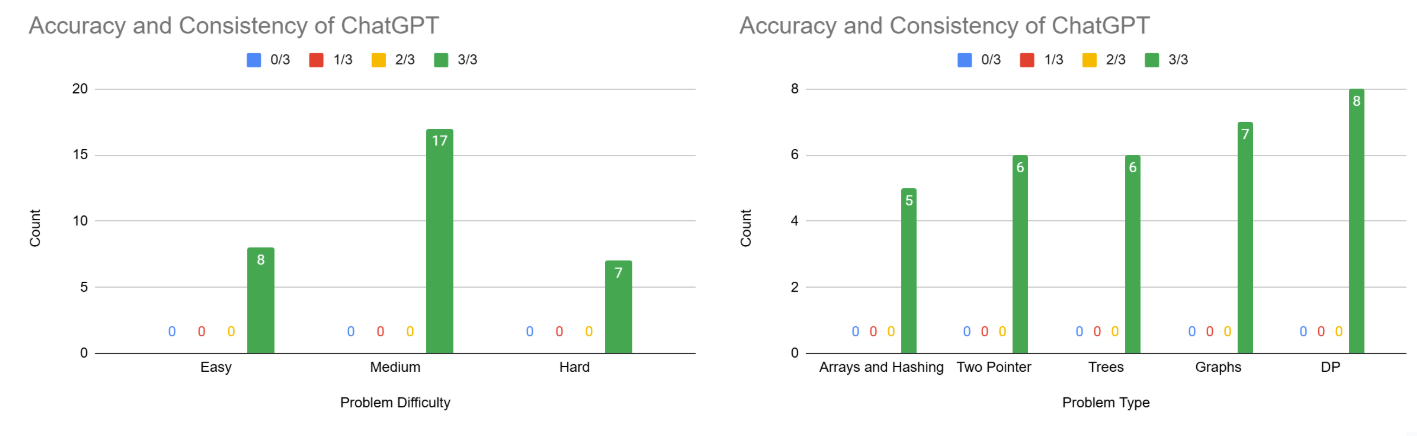
\includegraphics[width=\textwidth]{imgs/chat.png} % Replace with your image file
        \caption{Accuracy and Consistency of ChatGPT4o}
        \label{fig:sub1}
    \end{subfigure}
    \hfill
    % Second subfigure
    \begin{subfigure}[b]{0.45\textwidth}
        \centering
        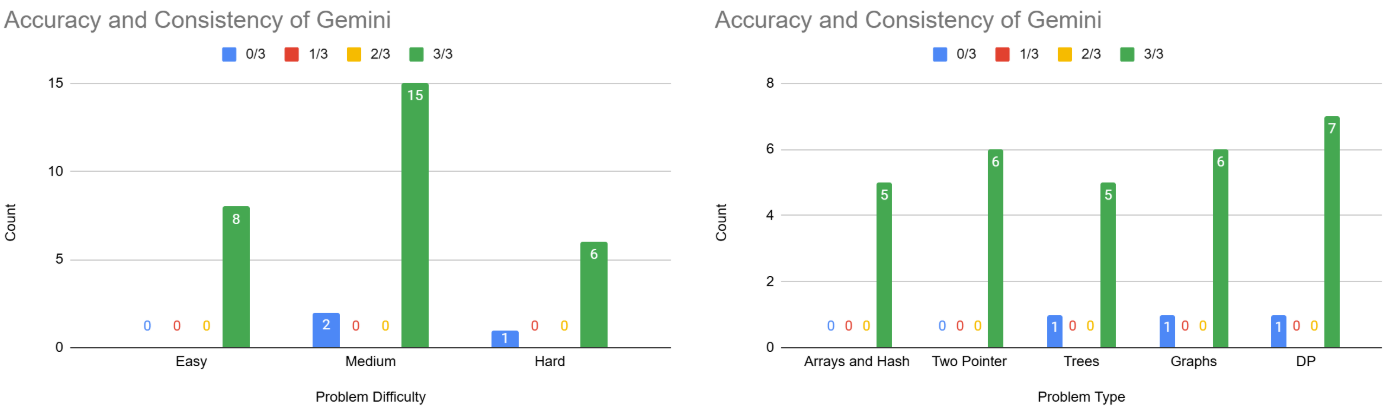
\includegraphics[width=\textwidth]{imgs/gemini.png} % Replace with your image file
        \caption{Accuracy and Consistency of Gemini 1.5 Flash}
        \label{fig:sub2}
    \end{subfigure}
    \hfill
    % Third subfigure
    \begin{subfigure}[b]{0.45\textwidth}
        \centering
        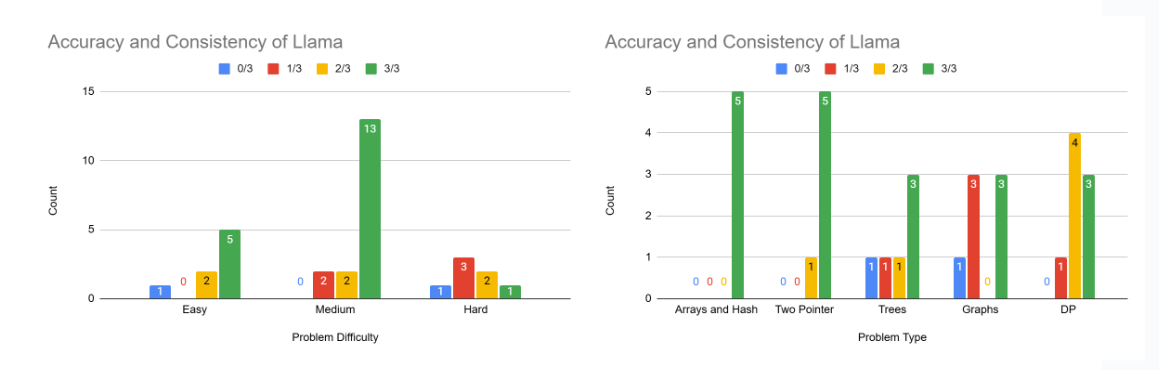
\includegraphics[width=\textwidth]{imgs/llama.png} % Replace with your image file
        \caption{Accuracy and Consistency of Llama 3 8B}
        \label{fig:sub3}
    \end{subfigure}
    % Overall caption
    \caption{Accuracy Results for all 3 models}
    \label{fig:main}
\end{figure}


The results of our experiment can be seen in Figure~\ref{fig:main}. Figure~\ref{fig:sub1} shows the accuracy and consistency of the code generated for each Leetcode question for ChatGPT-4o. This model was able to provide code that passed all of the given test cases for each of the 3 trials that were performed for each problem, regardless of the difficulty level or problem categorization.

Figure~\ref{fig:sub2} shows the results for Gemini Flash 1.5. The results for this model were comparable to the results from ChatGPT-4o, with only 3 incorrect solutions out of the 32 problems that were being tested. An interesting thing to note for this model is that the responses were consistent, even in its wrong answers. For the problems Gemini 1.5 Flash was unable to provide a correct solution for, it produced an incorrect response for all 3 trials, with each response generating the same error in the IDE. 

The results for the last model, Llama 3 8B, can be seen in Figure~\ref{fig:sub3}. As shown in the graphs, there are far more variations or inconsistencies in the results from this model.
It was able to generate correct solutions for most of medium- and easy-level questions, but the hard-level questions resulted in more incorrect solutions. This is probably due to the fact that hard questions are more nuanced and have more edge cases to be aware of that the model was not able to capture in its code. In terms of problem category,
Arrays/Hashing and Two-pointer questions were answered more accurately, and this is likely because these questions typically more widespread and easier to answer than Trees, Graphs, and DP problems. 

\subsection{Problem Categorization Accuracy}

\begin{figure}[h]
    \centering
    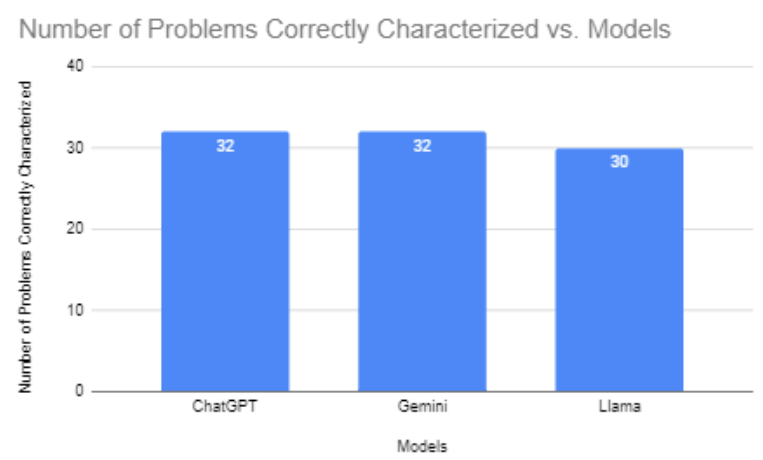
\includegraphics[width=0.45
    \textwidth]{imgs/categorization_all3.png} % Replace 'example.jpg' with your image file
    \caption{Results for problem categorization}
    \label{fig:example} % Label for referencing
\end{figure}

Figure \ref{fig:example} shows the results for problem categorization for each of the 3 models. Overall, all 3 models were able to categorize most, if not all, of the 32 questions that were tested. The model with the lowest accuracy was LLama 3 8B, with an accuracy of 30/32. 

\subsection{Accuracy and Consistency on Mutated Problems}

\begin{figure}[h]
    \centering
    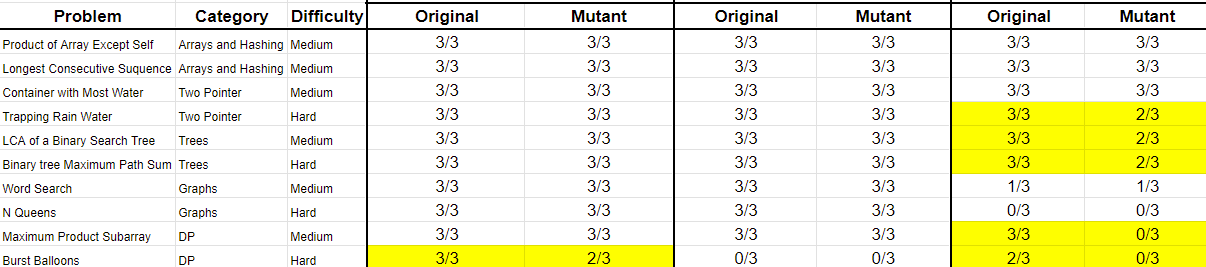
\includegraphics[width=0.45
    \textwidth]{imgs/mutant-testing.png} % Replace 'example.jpg' with your image file
    \caption{Results for Mutation Testing}
    \label{fig:mutation} % Label for referencing
\end{figure}

Mutation testing was performed on all 3 models in order to test their generalizability or adaptability, in the case that the exact versions of the LeetCode problems were present in the training dataset and already seen by the models during training. As seen in Figure~\ref{fig:mutation}, Gemini 1.5 Flash produced the same results as the original problems, whereas ChatGPT-4o and Llama 3 8B saw a decrease in accuracy, with a far a larger decrease for LLama 3 8B. This could be attributed to ChatGPT-4o and Gemini 1.5 Flash being more fine-tuned or optimized for programming tasks compared to Llama 3 8B, and are better at adapting to variations in problem definitions due to their larger model size and refined architecture. 


\subsection{Analysis of Results}
For our experiment, we saw that models with more parameters (ChatGPT-4o and Gemini 1.5 Flash) performed better overall than models with less parameters (Llama 3 8B). Within the scope of our project, we were able to conclude that there may be a correlation between model size and the ability to generate accurate and consistent solutions for DSA problems. However, one thing to consider is that Gemini 1.5 Flash is a more lightweight model that was trained through model distillation from larger models (with sizes comparable to ChatGPT-4o). Gemini 1.5 Flash therefore has far fewer parameters than ChatGPT-4o, but has relatively comparable results. Therefore, though model size may impact performance, there is not a linear correlation between number of parameters and accuracy. Other factors may also play a role in model performance, such as model architecture, training time/methodologies, training data, context window, etc. 

Additionally, we noticed that ChatGPT-4o and Gemini 1.5 Flash occasionally cited websites such as GitHub or LeetCode itself in its responses, which is an indication that these models utilize Retrieval Augmented Generation (RAG). More advanced models are known to combine traditional querying/document retrieval with generative AI, which may also be a reason for their improved performance.


\Section{Conclusion and Future Work}
Our study reveals that larger and more refined Large Language Models (LLMs) like ChatGPT-4o and Gemini 1.5 Flash outperform smaller models such as Llama 3 8B on Data Structures and Algorithms (DSA) problems. These bigger models are more accurate, consistent, and better at handling variations in problem statements. Interestingly, Gemini 1.5 Flash, despite having fewer parameters than ChatGPT-4o, performed just as well, highlighting that factors like model design and training techniques matter a lot.

For future research, it would be valuable to test a wider range of models, especially those specifically designed for coding tasks. Trying these models on more complex and varied problems, including real-world software development challenges, could offer deeper insights. Additionally, looking into how efficient these models are in terms of resource use could help assess their practicality for everyday applications.

In summary, while LLMs show great promise in solving coding problems, there's still a gap between their current abilities and the full spectrum of software engineering tasks. This work is a step toward understanding how these models can contribute to the future of programming and automation.   

Here is the link to the GitHub \textbf{\href{https://github.com/JaykumarPatel4802/software-testing-project}{repository}} that contains the prompts, problem formulations, and mutation formulations. Here is the link to the Google Sheets \textbf{\href{https://docs.google.com/spreadsheets/d/11I5tJY4y23TiVjcQp0gYHosABqDVvtIG0WB7ye1b420/edit?usp=sharing}{spreadsheet}} that contains the results of our experiments.

%------------------------------------------------------------------------- 
% \nocite{ex1,ex2}
\bibliographystyle{latex8}
\bibliography{latex8}

\pagebreak

\end{document}

